\documentclass[border=6pt]{standalone}
\usepackage{tikz}
\usetikzlibrary{positioning,arrows.meta,shapes.geometric,calc}
\usepackage[T1]{fontenc}
\usepackage{helvet}
\renewcommand{\familydefault}{\sfdefault}

\definecolor{ink}{HTML}{1F2933}
\definecolor{seg}{HTML}{E8F1FB}
\definecolor{segb}{HTML}{2E6DA4}
\definecolor{ins}{HTML}{EAF5EC}
\definecolor{insb}{HTML}{2F7D4F}
\definecolor{ev}{HTML}{FFF4E0}
\definecolor{evb}{HTML}{B7791F}
\definecolor{val}{HTML}{FDEBEC}
\definecolor{valb}{HTML}{A33A3A}
\definecolor{rep}{HTML}{F1ECF7}
\definecolor{repb}{HTML}{6B4C9A}

\tikzset{
  box/.style 2 args={
    draw=#1, fill=#2, line width=0.7pt, rounded corners=3pt,
    align=center, text=ink, font=\scriptsize, inner sep=3pt,
    minimum height=1.0cm, text width=2.3cm
  },
  flow/.style={-{Latex[length=2.0mm,width=1.5mm]}, line width=0.8pt, draw=ink!75},
  tag/.style={font=\scriptsize\bfseries, text=ink!75, align=center}
}

\begin{document}
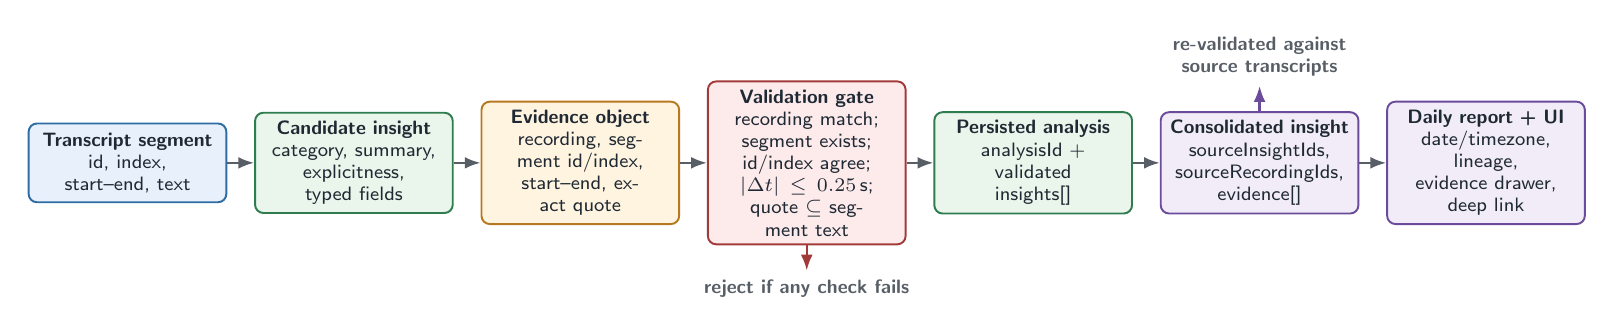
\begin{tikzpicture}[node distance=0.34cm]

\node[box={segb}{seg}] (seg) {\textbf{Transcript segment}\\ id, index,\\ start--end, text};
\node[box={insb}{ins}, right=of seg] (cand) {\textbf{Candidate insight}\\ category, summary,\\ explicitness, typed fields};
\node[box={evb}{ev}, right=of cand] (evid) {\textbf{Evidence object}\\ recording, segment id/index,\\ start--end, exact quote};
\node[box={valb}{val}, right=of evid] (gate) {\textbf{Validation gate}\\ recording match; segment exists;\\ id/index agree; $|\Delta t|\le0.25$\,s;\\ quote $\subseteq$ segment text};
\node[box={insb}{ins}, right=of gate] (analysis) {\textbf{Persisted analysis}\\ analysisId + validated\\ insights[]};
\node[box={repb}{rep}, right=of analysis] (cons) {\textbf{Consolidated insight}\\ sourceInsightIds,\\ sourceRecordingIds,\\ evidence[]};
\node[box={repb}{rep}, right=of cons] (report) {\textbf{Daily report + UI}\\ date/timezone, lineage,\\ evidence drawer, deep link};

\draw[flow] (seg) -- (cand);
\draw[flow] (cand) -- (evid);
\draw[flow] (evid) -- (gate);
\draw[flow] (gate) -- (analysis);
\draw[flow] (analysis) -- (cons);
\draw[flow] (cons) -- (report);

% rejected candidate annotation
\node[tag, below=0.32cm of gate] (reject) {reject if any check fails};
\draw[flow, draw=valb] (gate.south) -- (reject.north);

% reuse annotation
\node[tag, above=0.32cm of cons] (reuse) {re-validated against\\ source transcripts};
\draw[flow, draw=repb] (cons.north) -- (reuse.south);

\end{tikzpicture}
\end{document}
